\section{Zielsetzung}
\label{sec:Zielsetzung}
In diesem Versuch werden Brückenschaltungen dazu verwendet verschiedene unbekannte Ohm'sche Widerstände, Kapazitäten und Induktivitäten
zu bestimmen. Zudem wird die Wien-Robinson-Brücke dazu verwendet um die Frequenzabhängigkeit dieser Schaltung zu untersuchen. \\
Dabei werden bisher nur in der Theorie benutze Konzepte angewendet, wie beispielsweise die Abgleichbedingung und die Kirchhoff'schen Gesetze.

\section{Theorie}
\label{sec:Theorie}

Brückenschaltungen werden dazu benutzt, durch bereits bekannte Widerstände Unbekannte zu bestimmen. Zu diesen Widerständen zählen
Ohm'sche Widerstände, induktive Widerstände und kapazitative Widerstände. Bei den letzteren Beiden handelt es sich um komplexe
Widerstände. \\
Allgemein werden bei allen folgenden Schaltungen die Kirchhoffschen Gesetze verwendet. Das Erste besagt, dass die Summe aller eingehenden
und ausgehenden Ströme an einem Knoten Null ist:
\begin{equation}
    \sum_k I_k = 0 \\ \label{eqn:K1}
\end{equation}
Das Zweite besagt, dass die Summe aller Speisespannungen gleich der Summe der Produkte der Stromstärken und Widerständen innerhalb einer Masche ist:
\begin{equation}
    \sum_k U_k = \sum_k I_k R_k \label{eqn:K2}
\end{equation}
Bei \autoref{eqn:K2} werden alle $I_k$ im Uhzeigersinn als positiv und alle gegen den Uhzeigersinn als negativ gewertet. \\
Aus diesen grundlegenden Gesetzten (\autoref{eqn:K1} und \autoref{eqn:K2}) lässt sich die Abgleichbedingung herleiten:
\begin{equation*}
    U_{Br} = \frac{R_2 R_3 - R_1 R_4}{(R_3 + R_4)(R_1 + R_2)} U_S
\end{equation*}
Wenn nun die Brückenspannung verschwindet, ergibt sich:
\begin{equation}
    R_1 R_4 = R_2 R_3 \label{eqn:Abgl}
\end{equation}
\\

\subsection{Wheatstonesche Brückenschaltung}
 
Der einfachste Aufbau einer Brückenschaltung besteht aus einer Speisespannung $U_S$, drei bekannten und einem unbekannten Ohm'schen Widerstand und
einem Spannungsmessgerät, was wie in \autoref{Abb:Wheatstone} aufgebaut wird.

\begin{figure}
    \centering
    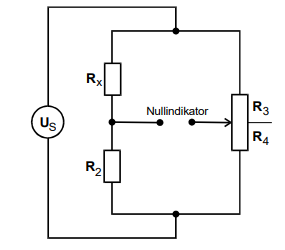
\includegraphics{Wheatstone.png}
    \caption{Wheatstonesche Brückenschaltung \cite{Blatt}}
    \label{Abb:Wheatstone}
\end{figure}

Bei \autoref{Abb:Wheatstone} handelt es sich um eine Wheatstonesche Brückenschaltung. Sie kann sowohl mit Gleichstrom, als auch mit Wechselstrom betrieben werden.
Diese Schaltung wird zur Bestimmung des Ohm'schen Widerstands $R_X$ benutzt. Die Widerstände $R_3$ und $R_4$ können in diesem Fall durch ein Potentiometer ersetzt werden,
da nur das Verhätnis der beiden Widerstände relevant zur Bestimmung von $R_X$ ist. \\
Mit \autoref{eqn:Abgl} wird nun eine Formel für $R_X$ bestimmt:
\begin{equation}
    R_X = R_2 \frac{R_3}{R_4} \label{eqn: RXW}
\end{equation}
Da diese Formel nur erfüllt ist, wenn die Brückenspannung Null ist, wird das Potentiometer [Verhätnis von $R_3$ und $R_4$] angepasst, bis die
mit dem Spannungsmessgerät gemessene Spannung verschwindet.

\subsection{Kapazitätsmessbrücke}

\begin{figure}
    \centering
    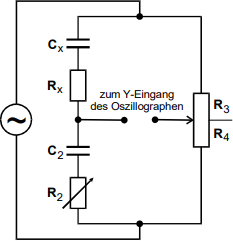
\includegraphics{Kapazitätsmessbrücke.png}
    \caption{Kapazitätsmessbrücke \cite{Blatt}}
    \label{Abb:Kapazitaetsmessbruecke}
\end{figure}


Bei der Kapazitätsmessbrücke wird grundlegend derselbe Aufbau verwendet wie bei \autoref{Abb:Wheatstone}. Da Kondensatoren einen Teil der durchfließenden 
elektrischen Energie in Wärme umwandeln, wird ein Ersatzschaltbild verwendet. Die dielektrischen Verluste werden durch einen mit dem Kondensator in Reihe geschalteten
fiktiven Ohm'schen Widerstand dargestellt. Der reale Widerstand des Kondensators berechnet sich also aus:
\begin{equation*}
    Z_{C_{real}} = R - \frac{j}{\omega C}
\end{equation*}
In dem Aufbau \autoref{Abb:Kapazitaetsmessbruecke} der Brückenschaltung wird zudem ein zweiter Abstimmfreiheitsgrad ($R_2$) gewählt, um die durch $R_X$ 
auftretende Phasenverschiebung zu kompensieren.
Die beiden Unbekannten berechnen sich dann mit \autoref{eqn:Abgl} folgendermaßen:
\begin{equation}
    R_X = R_2 \frac{R_3}{R_4} \label{eqn:CRX}
\end{equation}
\begin{equation}
    C_X = C_2 \frac{R_4}{R_3} \label{eqn:CCX}
\end{equation}

\subsection{Induktivitätsmessbrücke}

\begin{figure}
    \centering
    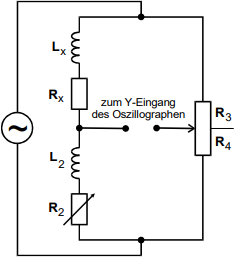
\includegraphics{Induktivitätsmessbrücke.png}
    \caption{Induktivitätsmessbrücke \cite{Blatt}}
    \label{Abb:Induktivitaetsmessbruecke}
\end{figure}

Die Spule hat genau dasselbe Problem wie der Kondensator. Sie setzt einen Teil der magnetischen Feldenergie irreversibel in Wärme. Daher wird wie beim Kondensator
ein Ersatzschaltbild mit einem Ohm'schen Widerstand verwendet. Der Aufbau \autoref{Abb:Induktivitaetsmessbruecke} bleibt derselbe wie bei \autoref{Abb:Kapazitaetsmessbruecke}.
Der reale Widerstand der Spule setzt sich folgendermaßen zusammen:
\begin{equation*}
    Z_{L_{real}} = R + j \omega L
\end{equation*}
 
Analog zu \autoref{eqn:CRX} und \autoref{eqn:CCX} lassen sich die jeweils gesuchten Größen so formulieren:

\begin{equation}
    R_X = R_2 \frac{R_3}{R_4} \label{eqn:LRX}
\end{equation}
\begin{equation}
    L_X = L_2 \frac{R_4}{R_3} \label{eqn:LLX}
\end{equation}

Wie auch bei der Kapazitätsmessbrücke wird hier der Widerstand $R_2$ variabel gewählt, um der durch $R_X$ verursachten Phasenverschiebung entgegen zu wirken.

\subsection{Maxwell-Brücke}

\begin{figure}
    \centering
    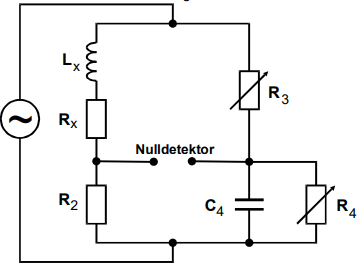
\includegraphics{Maxwell.png}
    \caption{Maxwell-Brücke \cite{Blatt}}
    \label{Abb:Maxwell}
\end{figure}

Eine weitere Möglichkeit eine unbekannte Induktivität zu bestimmen besteht durch die Maxwell-Brückenschaltung. Der Unterschied zu allen bisherigen Schaltungen liegt darin,
dass bei keiner der Abgleichbedingungen die Frequenz der Speisespannung mit einging.\\
Der Aufbau der Schaltung \autoref{Abb:Maxwell} ist wieder ähnlich zu \autoref{Abb:Induktivitaetsmessbruecke}. Allerdings werden anstelle des Potentiometer die Widerstände $R_3$ und $R_4$ variabel
gewählt. Zudem wird parallel zu $R_4$ ein bekannter Kondensator geschaltet.\\
Mit der Abgleichbedingung ergeben sich nun folgende Formeln für die gesuchten Größen:

\begin{equation}
    R_X = R_2 \frac{R_3}{R_4} \label{eqn:LCRX}
\end{equation}
\begin{equation}
    L_X = R_2 R_3 C_4 \label{eqn:LLCX}
\end{equation}
\\
\\
\\
\\
\subsection{Wien-Robinson-Brücke}

\begin{figure}
    \centering
    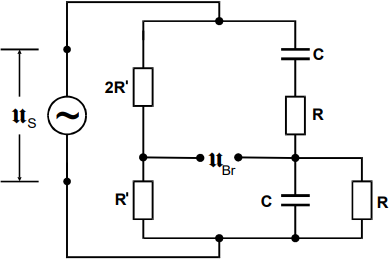
\includegraphics{Wien.png}
    \caption{Wien-Robinson-Brücke \cite{Blatt}}
    \label{Abb:Wien}
\end{figure}

Die Wien-Robinson-Brücke hat im Gegensatz zu den anderen keine Abgleichelemente und ist eine frequenzabhängige Brückenschaltung. Sie wird
nicht zur Bestimmung von Widerständen verwendet, sondern als elektrischer Filter. Mithilfe dieser Schaltung soll im Rahmen des Versuchs die
Frequenzabhängigkeit der Speisespannung und der Brückenspannung gemessen werden.
Die Brückenspannung wird folgendermaßen bestimmt:
\begin{equation}
    U_{Br} = \frac{\omega ^2 R^2 C^2 - 1}{3(1- \omega ^2 R^2 C^2) + 9 j \omega RC}U_S
\end{equation}
Durch teilen von $U_S$ und quadrieren ergibt sich folgende Formel:
\begin{equation}
    \biggl|\frac{U_{Br}}{U_S}\biggl|^2 = \frac{(\omega ^2 R^2 C^2 - 1)^2}{9[(1- \omega ^2 R^2 C^2)^2 + 9 \omega^2 R^2C^2]} \label{eqn:Ubr/Us}
\end{equation}
Anhand \autoref{eqn:Ubr/Us} erkennt man gut, dass die Brückenspannung verschwindet wenn $\omega_0 = \frac{1}{RC}$ ist. Wir wählen zudem $\Omega := \frac{\omega}{\omega_0}$.
Damit verkürzt sich \autoref{eqn:Ubr/Us} zu:
\begin{equation}
    \biggl|\frac{U_{Br}}{U_S}\biggl|^2 = \frac{(\Omega ^2 - 1)^2}{9[(1-\Omega ^2)^2 + 9 \Omega ^2]} \label{eqn:Omega}
\end{equation}
Die Wien-Robinson-Brücke filtert aus einem kontinuierlichen Frequenzspektrum Schwingungen mit $\omega_0 = \frac{1}{RC}$ und schwächt die in nächster Nähe stark. Dadurch
könnten ebenfalls Widerstände oder Kapazitäten bestimmt werden.
\newpage